\documentclass[11pt]{article}

\usepackage[margin=0.9in]{geometry}
\usepackage[T1]{fontenc}
\usepackage{lmodern}
\usepackage{microtype}
\usepackage{amsmath,amssymb}
\usepackage{booktabs}
\usepackage{graphicx}
\usepackage{float}
\usepackage{xcolor}
\usepackage{hyperref}
\usepackage{enumitem}
\usepackage{caption}

\hypersetup{
  colorlinks=true,
  linkcolor=blue!55!black,
  urlcolor=blue!55!black,
  citecolor=blue!55!black
}

\graphicspath{{../../}{./}}

\newcommand{\code}[1]{\texttt{\detokenize{#1}}}
\newcommand{\cp}{c_{+}}
\newcommand{\cn}{c_{-}}
\newcommand{\ph}{\phi}
\newcommand{\Dp}{D_{+}}
\newcommand{\Dn}{D_{-}}
\newcommand{\Jp}{J_{+}}
\newcommand{\Jn}{J_{-}}

\setlist[itemize]{topsep=3pt,itemsep=2pt,leftmargin=1.25em}
\setlist[enumerate]{topsep=3pt,itemsep=2pt,leftmargin=1.35em}

\title{\vspace{-2em}\textbf{Project Technical Note}\\
\large Parameterized PINN for Current-Based Inference in a 1D PNP Model}
\author{Jack Jia}
\date{May 31, 2026}

\begin{document}
\maketitle

\section*{Short Version}

This project builds a parameterized PINN surrogate for a one-dimensional
Poisson--Nernst--Planck (PNP) model. The trained network takes
\[
  (x,t,\Dp,\Dn)
\]
as input and predicts
\[
  (\cp,\cn,\ph),
\]
where $\cp$ and $\cn$ are ion concentrations, $\ph$ is electric potential, and
$\Dp,\Dn$ are the diffusion parameters we want to infer.

The current goal is not just to solve the PDE once. The goal is to use the PINN
as a fast reusable forward model inside an inverse problem. We generate
synthetic electrode charging-current data from an independent finite-difference
reference solver, add Gaussian noise, and then use the trained PINN to infer the
posterior distribution of $\Dp$ and $\Dn$.

\section*{What I Am Modeling}

The physical model is a nondimensional 1D binary-electrolyte PNP system on
\[
  x\in[0,1],\qquad t\in[0,0.2],\qquad \Dp,\Dn\in[0.5,2.0].
\]

The two ion fluxes are
\[
  \Jp = -\Dp\,\partial_x\cp - \Dp z_+\cp\,\partial_x\ph,
\]
\[
  \Jn = -\Dn\,\partial_x\cn - \Dn z_-\cn\,\partial_x\ph,
\]
with
\[
  z_+=1,\qquad z_-=-1,\qquad \epsilon=1.
\]

The PDE residuals are:
\[
  \partial_t\cp+\partial_x\Jp=0,
\]
\[
  \partial_t\cn+\partial_x\Jn=0,
\]
\[
  -\epsilon\,\partial_{xx}\ph-(z_+\cp+z_-\cn)=0.
\]

The initial and boundary conditions are:
\[
  \cp(x,0)=1,\qquad \cn(x,0)=1,
\]
\[
  \ph(0,t)=-0.5,\qquad \ph(1,t)=0.5,
\]
\[
  \Jp(0,t)=\Jp(1,t)=0,\qquad \Jn(0,t)=\Jn(1,t)=0.
\]

This is a blocking-electrode setup. Ions do not pass through the boundaries.
The current signal used later is therefore charging current, not ionic flux
through the wall.

\section*{Why This Setup Is Reasonable}

This is a clean benchmark model, not a full experimental electrochemical cell.
The no-flux ion boundary is not arbitrary: it corresponds to blocking
electrodes, where the electrolyte charges capacitively but there is no Faradaic
reaction at the wall.

The most idealized part is the electrode interface. In a real experiment, the
interface may include Stern-layer capacitance, Faradaic kinetics, adsorption,
leakage current, and external circuit effects. I am not modeling those yet. The
current benchmark is meant to test whether a trained PINN surrogate can support a
controlled current-based inverse problem.

\section*{What The PINN Learns}

The network learns the parameterized map
\[
  (x,t,\Dp,\Dn)\mapsto(\cp,\cn,\ph).
\]

The active model is an Equinox MLP:
\[
\begin{array}{ll}
\text{input dimension} & 4 \\
\text{output dimension} & 3 \\
\text{width} & 256 \\
\text{depth} & 8 \\
\text{activation} & \tanh
\end{array}
\]

The model uses hard constraints for the most important fixed-value conditions.
For concentration:
\[
  \cp = 1 + t\,r_+,\qquad \cn = 1 + t\,r_-.
\]
So the concentration initial condition is exact.

For electric potential:
\[
  \ph = \ph_{\mathrm{wall}}(x) + 4\xi(1-\xi)r_\ph.
\]
The factor $4\xi(1-\xi)$ is zero at both walls, so the wall voltages are exact.

\section*{How The PINN Is Trained}

Each training step samples three groups of collocation points:

\begin{itemize}
  \item interior domain points for the PNP residuals,
  \item boundary-layer points near the two walls,
  \item wall points for no-flux boundary residuals.
\end{itemize}

The loss has three groups:
\[
  \mathcal{L}
  =
  w_{\mathrm{dom}}\mathcal{L}_{\mathrm{dom}}
  +
  w_{\mathrm{bl}}\mathcal{L}_{\mathrm{bl}}
  +
  w_{\mathrm{bc}}\mathcal{L}_{\mathrm{bc}}.
\]

The group weights are adjusted during training with an NTK-style balancing rule.
Training uses Adam on the CPU backend. CPU is used because the nested automatic
differentiation in this PINN is stable there on the local Apple M4 environment.

\section*{Current Trained Run}

The main trained run is:

\begin{verbatim}
checkpoints/runs/pnp_1d_hard_phi_high_quality_20260527_074537
\end{verbatim}

It completed 500,000 steps. The main training summary is:

\begin{center}
\begin{tabular}{lr}
\toprule
Metric & Value \\
\midrule
Final loss & $1.236948\times 10^{-2}$ \\
Final domain loss & $2.227460\times 10^{-3}$ \\
Final boundary-layer loss & $5.163684\times 10^{-3}$ \\
Final boundary loss & $7.020860\times 10^{-3}$ \\
Best logged loss & $3.645345\times 10^{-3}$ \\
Final step & 500,000 \\
Training time & about 8 h 9 m \\
\bottomrule
\end{tabular}
\end{center}

\section*{How I Check The Forward Model}

There are two levels of forward diagnostics.

\subsection*{Phase A: PINN-only checks}

These checks evaluate whether the trained PINN obeys the constraints and basic
physical sanity checks.

\begin{center}
\begin{tabular}{lr}
\toprule
Check & Result \\
\midrule
Wall-voltage error & 0 \\
$\cp(x,0)-1$ max error & 0 \\
$\cn(x,0)-1$ max error & 0 \\
Minimum $\cp$ on diagnostic grid & 0.5867 \\
Minimum $\cn$ on diagnostic grid & 0.5894 \\
Maximum $\cp$ mass drift & $1.61\times10^{-3}$ \\
Maximum $\cn$ mass drift & $3.25\times10^{-3}$ \\
\bottomrule
\end{tabular}
\end{center}

\subsection*{Phase B: comparison to reference solver}

The reference solver is independent of the PINN. It is a finite-difference
method-of-lines solver:

\begin{itemize}
  \item Poisson's equation is solved by a banded linear solve.
  \item The ion fluxes are computed on spatial faces.
  \item Time integration uses SciPy's BDF solver.
\end{itemize}

At $n_x=401$, the PINN-reference comparison is:

\begin{center}
\begin{tabular}{rrrrr}
\toprule
$\Dp$ & $\Dn$ & $\cp$ rel. $L^2$ & $\cn$ rel. $L^2$ & $\ph$ rel. $L^2$ \\
\midrule
1.25 & 1.25 & $8.493\times10^{-4}$ & $5.090\times10^{-4}$ & $2.499\times10^{-2}$ \\
0.50 & 0.50 & $1.575\times10^{-3}$ & $1.186\times10^{-3}$ & $1.689\times10^{-2}$ \\
2.00 & 2.00 & $8.223\times10^{-4}$ & $6.199\times10^{-4}$ & $2.796\times10^{-2}$ \\
0.50 & 2.00 & $3.304\times10^{-3}$ & $2.580\times10^{-3}$ & $2.604\times10^{-2}$ \\
2.00 & 0.50 & $5.664\times10^{-4}$ & $1.080\times10^{-3}$ & $2.675\times10^{-2}$ \\
\bottomrule
\end{tabular}
\end{center}

The concentrations match very well. The potential error is larger, but still
small enough for the current inverse demonstration.

\section*{The Inverse Problem}

The inverse problem is:

\begin{quote}
Given noisy current measurements, infer the posterior distribution of
$\Dp$ and $\Dn$.
\end{quote}

The workflow is:

\begin{enumerate}
  \item Pick true parameters, here $\Dp=1.25$, $\Dn=1.25$.
  \item Use the finite-difference/BDF reference solver to generate clean
        charging-current data.
  \item Add independent Gaussian noise.
  \item Use the trained PINN to predict current for candidate parameter pairs.
  \item Compare predicted current to observed current through a Gaussian
        likelihood.
  \item Normalize the likelihood over a parameter grid to obtain the posterior.
\end{enumerate}

\section*{What Current Means Here}

Because the boundary is no-flux, the boundary ionic flux current is zero. That
is not the current used here.

The current used here is electrode charging current. First compute the electrode
charge response $Q(t)$, then use interval-averaged current:
\[
  I_k = \frac{Q(t_{k+1})-Q(t_k)}{t_{k+1}-t_k}.
\]

For the exact PNP solution, electrode charge can be written in terms of the wall
electric field. For the PINN evaluation, I use an equivalent Gauss-law integral
over charge density. This is more stable because it avoids taking a boundary
derivative of the neural-network potential.

\section*{Likelihood}

The observation model is:
\[
  I^{\mathrm{obs}}_k = I^{\mathrm{PINN}}_k(\Dp,\Dn) + \varepsilon_k,
\]
where
\[
  \varepsilon_k\sim \mathcal{N}(0,\sigma^2).
\]

For this synthetic experiment:
\[
  \sigma = 0.02 \times \max_k |I^{\mathrm{clean}}_k|.
\]

In this run:
\[
  \sigma = 0.0418868.
\]

So the likelihood is:
\[
  p(I^{\mathrm{obs}}\mid \Dp,\Dn)
  =
  \prod_k
  \mathcal{N}
  \left(
    I^{\mathrm{obs}}_k ;
    I^{\mathrm{PINN}}_k(\Dp,\Dn),
    \sigma^2
  \right).
\]

The prior is uniform on:
\[
  \Dp,\Dn\in[0.5,2.0].
\]

The posterior is evaluated on a $41\times41$ grid.

\section*{Current-Based Inference Result}

The current-based inference output is:

\begin{verbatim}
checkpoints/runs/pnp_1d_hard_phi_high_quality_20260527_074537/
diagnostics/phase_c_current_probe
\end{verbatim}

The result is:

\begin{center}
\begin{tabular}{lr}
\toprule
Quantity & Value \\
\midrule
True $\Dp$ & 1.25 \\
True $\Dn$ & 1.25 \\
MAP $\Dp$ & 1.25 \\
MAP $\Dn$ & 1.2125 \\
Posterior mean $\Dp$ & 1.23531 \\
Posterior mean $\Dn$ & 1.23677 \\
95\% interval for $\Dp$ & $[1.0625, 1.4]$ \\
95\% interval for $\Dn$ & $[1.0625, 1.4375]$ \\
True value covered & yes \\
\bottomrule
\end{tabular}
\end{center}

\begin{figure}[H]
  \centering
  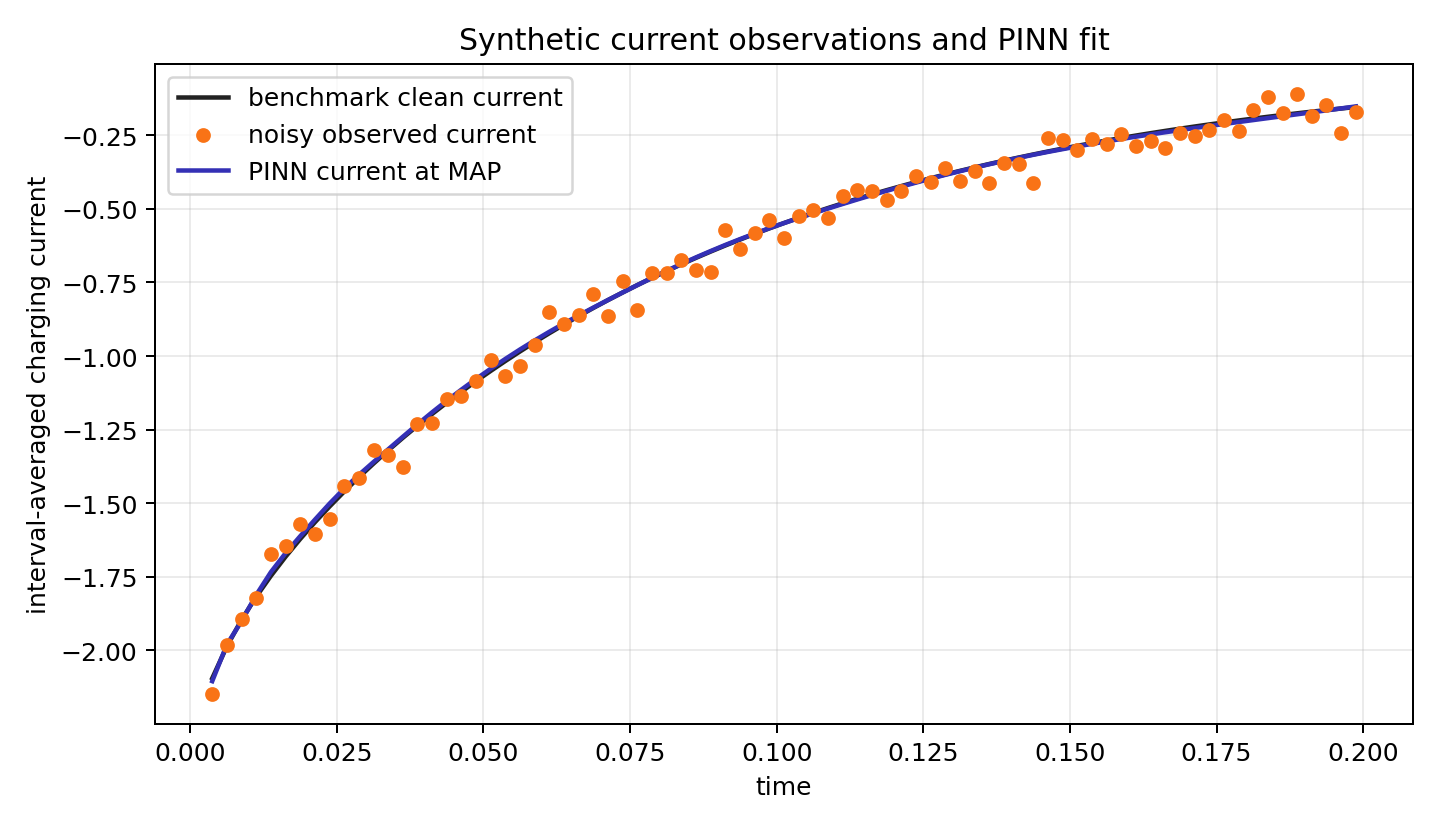
\includegraphics[width=0.9\textwidth]{checkpoints/runs/pnp_1d_hard_phi_high_quality_20260527_074537/diagnostics/phase_c_current_probe/current_fit.png}
  \caption{Clean benchmark current, noisy synthetic observations, and PINN current at the posterior MAP.}
\end{figure}

\begin{figure}[H]
  \centering
  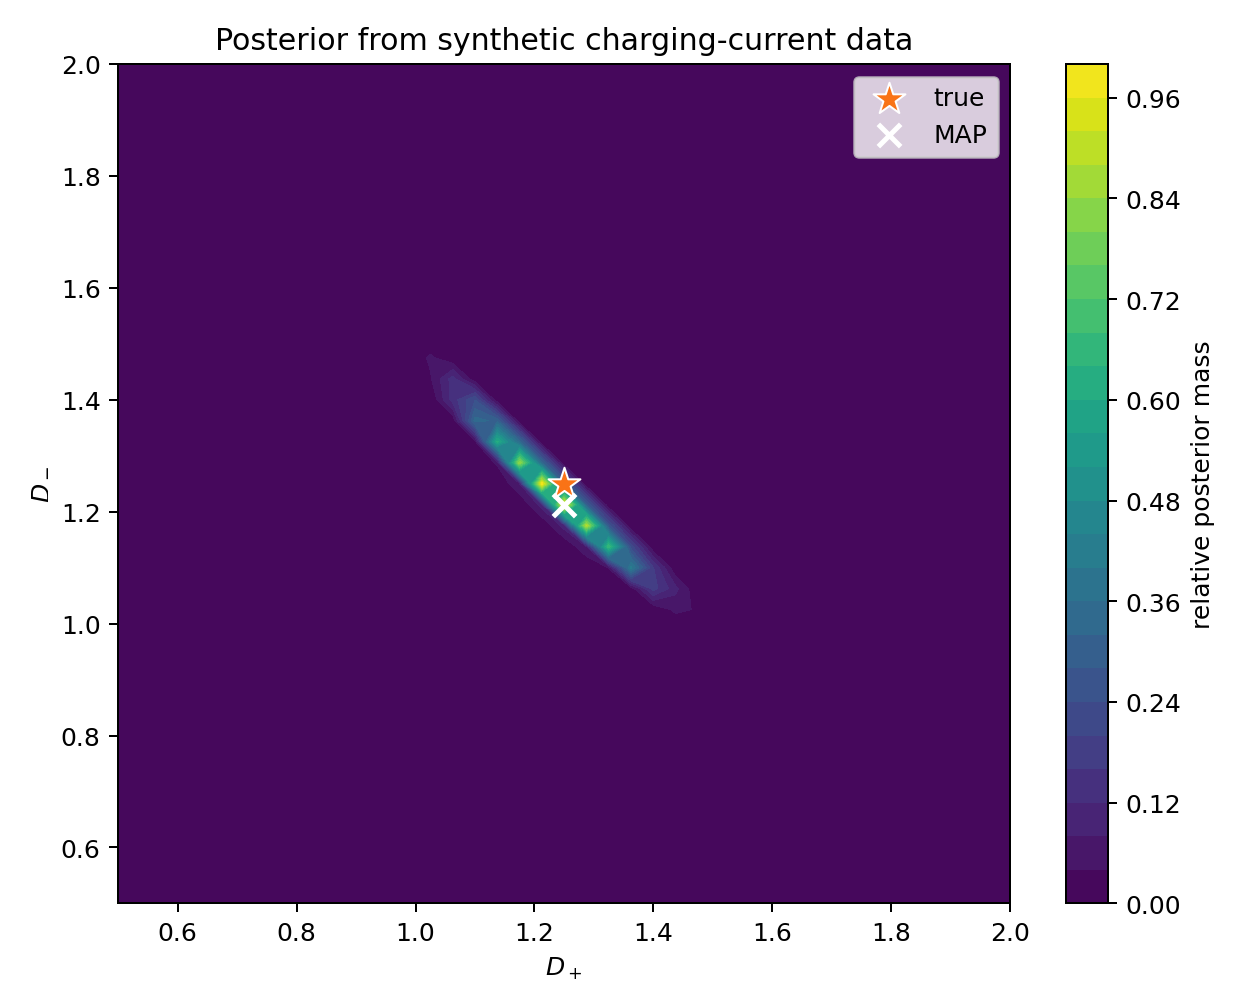
\includegraphics[width=0.72\textwidth]{checkpoints/runs/pnp_1d_hard_phi_high_quality_20260527_074537/diagnostics/phase_c_current_probe/posterior_contour.png}
  \caption{Posterior over $\Dp$ and $\Dn$ from synthetic charging-current observations.}
\end{figure}

\section*{What This Shows}

The main point is that direct concentration observations are not required for
the inverse problem. A compressed electrical signal, here charging current, can
still identify the diffusion parameters with uncertainty.

The posterior is not a point. It is an elongated region, which is useful:
current measurements identify a combination of $\Dp$ and $\Dn$ more strongly
than each parameter independently. This is exactly the kind of uncertainty
statement that a posterior distribution should reveal.

\section*{Why The PINN Is Useful}

The PINN is expensive to train, but cheap to reuse. The main trained run took
about 8 h 9 m. After that, repeated current predictions are much faster than
solving the reference PDE repeatedly.

Measured on this setup:

\begin{center}
\begin{tabular}{lr}
\toprule
Computation & Approximate time \\
\midrule
One finite-difference/BDF solve & 0.177 s \\
One PINN current evaluation in grid posterior & 0.004--0.006 s \\
Full $41\times41$ current posterior grid & 7.5 s \\
\bottomrule
\end{tabular}
\end{center}

For one prediction, the PINN is not worth the training cost. For many likelihood
evaluations, the cost can be amortized.

\section*{Limitations}

The important limitations are:

\begin{itemize}
  \item The model is 1D.
  \item The electrode interface is idealized.
  \item There are no Faradaic reactions.
  \item The current data are synthetic.
  \item The noise model is iid Gaussian.
  \item The posterior is computed on a grid rather than by MCMC.
\end{itemize}

These are acceptable for the current benchmark. The most natural extensions are
Stern-layer boundary conditions, Faradaic boundary kinetics, richer current
experiments, correlated noise, and MCMC posterior sampling.

\section*{Files To Check}

The most useful project files are:

\begin{itemize}
  \item \code{README.md}
  \item \code{src/pnp_pinn/model.py}
  \item \code{src/pnp_pinn/reference_solver.py}
  \item \code{src/pnp_pinn/current_observable.py}
  \item \code{scripts/run_current_probe.py}
  \item the run-level \code{RUN_SUMMARY.md}
  \item the current-probe \code{diagnostics/phase_c_current_probe/REPORT.md}
\end{itemize}

\section*{Bottom Line}

This project currently demonstrates a complete controlled pipeline:

\begin{quote}
train a parameterized PNP PINN, validate it against an independent numerical
solver, generate synthetic charging-current data, and infer $\Dp,\Dn$ through a
posterior distribution using the PINN as a fast forward surrogate.
\end{quote}

\end{document}
